%%%%%%%%%%%%%%%%%%%%%%%%%%%%%%%%%%%%%%%%%
% Beamer Presentation
% LaTeX Template
% Version 1.0 (10/11/12)
%
% This template has been downloaded from:
% http://www.LaTeXTemplates.com
%
% License:
% CC BY-NC-SA 3.0 (http://creativecommons.org/licenses/by-nc-sa/3.0/)
%
%%%%%%%%%%%%%%%%%%%%%%%%%%%%%%%%%%%%%%%%%

%----------------------------------------------------------------------------------------
%	PACKAGES AND THEMES
%----------------------------------------------------------------------------------------

\documentclass[a4paper,compress,svgnames]{beamer}

\mode<presentation> {

% The Beamer class comes with a number of default slide themes
% which change the colors and layouts of slides. Below this is a list
% of all the themes, uncomment each in turn to see what they look like.

%\usetheme{default}
%\usetheme{AnnArbor}
%\usetheme{Antibes}
%\usetheme{Bergen}
%\usetheme{Berkeley}
%\usetheme{Berlin}
%\usetheme{Boadilla}
%\usetheme{CambridgeUS}
%\usetheme{Copenhagen}
%\usetheme{Darmstadt}
%\usetheme{Dresden}
%\usetheme{Frankfurt}
%\usetheme{Goettingen}
%\usetheme{Hannover}
%\usetheme{Ilmenau}
%\usetheme{JuanLesPins}
%\usetheme{Luebeck}
\usetheme{Madrid}
%\usetheme{Malmoe}
%\usetheme{Marburg}
%\usetheme{Montpellier}
%\usetheme{PaloAlto}
%\usetheme{Pittsburgh}
%\usetheme{Rochester}
%\usetheme{Singapore}
%\usetheme{Szeged}
%\usetheme{Warsaw}

% As well as themes, the Beamer class has a number of color themes
% for any slide theme. Uncomment each of these in turn to see how it
% changes the colors of your current slide theme.

%\usecolortheme{albatross}
%\usecolortheme{beaver}
%\usecolortheme{beetle}
%\usecolortheme{crane}
%\usecolortheme{dolphin}
%\usecolortheme{dove}
%\usecolortheme{fly}
%\usecolortheme{lily}
%\usecolortheme{orchid}
%\usecolortheme{rose}
%\usecolortheme{seagull}
%\usecolortheme{seahorse}
%\usecolortheme{whale}
%\usecolortheme{wolverine}

%\setbeamertemplate{footline} % To remove the footer line in all slides uncomment this line
%\setbeamertemplate{footline}[page number] % To replace the footer line in all slides with a simple slide count uncomment this line

%\setbeamertemplate{navigation symbols}{} % To remove the navigation symbols from the bottom of all slides uncomment this line
}

\graphicspath{{figures/}}
\usepackage{graphicx} % Allows including images
\usepackage{booktabs} % Allows the use of \toprule, \midrule and \bottomrule in tables
\usepackage{commath} % For norm
\usepackage{multirow}
\usepackage{caption}
\usepackage[ruled,norelsize]{algorithm2e}
\usepackage{bm}
\usepackage{dirtree}
\usepackage{upgreek}


%-===========-MY ADDITIONS-======================
%gets rid of bottom navigation bars
\setbeamertemplate{footline}[page number]{}

%gets rid of navigation symbols
\setbeamertemplate{navigation symbols}{}


%----------------------------------------------------------------------------------------
%	TITLE PAGE
%----------------------------------------------------------------------------------------

\title[KM for DL]{A study on Deep Multi-layer Kernel Machines} % The short title appears at the bottom of every slide, the full title is only on the title page

\author{Akhil P M} % Your name
\institute[] % Your institution as it will appear on the bottom of every slide, may be shorthand to save space
{
Supervisor : Sumitra S. \\ % Your institution for the title page
%\medskip
%\textit{john@smith.com} % Your email address
}
\date{\today} % Date, can be changed to a custom date

\begin{document}

\begin{frame}
\titlepage % Print the title page as the first slide
\end{frame}

\begin{frame}
\frametitle{Overview} % Table of contents slide, comment this block out to remove it
\tableofcontents % Throughout your presentation, if you choose to use \section{} and \subsection{} commands, these will automatically be printed on this slide as an overview of your presentation
\end{frame}

%----------------------------------------------------------------------------------------
%	PRESENTATION SLIDES
%----------------------------------------------------------------------------------------
\begin{frame}
\frametitle{Multi-layer Kernels}
\setlength{\DTbaselineskip}{25pt}
\DTsetlength{1em}{1em}{0.1em}{1pt}{4pt}
\dirtree{%
.1 Multi-layer Kernels.
.2 Unsupervised Settings.
.3 Multi-layer Kernel Machines(MKMs).
.3 Multi-layer Multiple Kernel Learning(ML-MKL).
.2 Supervised Settings.
.3 Kernel Fisher Discriminant Analysis(KFDA).
.3 Multi-layer Kernels in Structured Output Spaces.
}
\end{frame}

%------------------------------------------------
\section{Multi-layer Kernels in Unsupervised Settings} % Sections can be created in order to organize your presentation into discrete blocks, all sections and subsections are automatically printed in the table of contents as an overview of the talk
%------------------------------------------------
\begin{frame}
\frametitle{Representation Learning}
Representation learning : a set of \textbf{preprocessing} of raw data, to produce a good representation of the data itself, which simplifies extracting useful information from the data when building classifiers or other predictors.\\
\vspace{0.1in}
Eg: dimensionality reduction, feature extraction, de-noising etc.\\
\vspace{0.3in}
An effective mechanism for transferring the \textbf{prior knowledge} of humans to the machine learning system.\\
\vspace{0.1in}
Eg: Sparse auto-encoders are formulated with the assumption of sparse representation of data in human brain.
\end{frame}

\begin{frame}
\frametitle{Representation Learning}
ML algorithms are broadly classified into two\\
\vspace{0.2in}
\begin{itemize}
\item Shallow architectures(eg: SVM, single hidden layer neural net, perceptron etc)
\item Deep Architectures(eq: deep learning algorithms like CNN, DBN etc.)
\end{itemize}
\end{frame}

\begin{frame}
\frametitle{Deep Learning}
Deep learning algorithms makes use of depth as a key criteria for producing good representations(hence they belong to deep architectures).\\
\vspace{0.2in}
\textit{Deep Learning is a set of algorithms in machine learning that attempts to model high-level abstractions in data by using model architectures composed of multiple non-linear transformations}.
\end{frame}

\begin{frame}
\frametitle{Deep Learning}
Deep Learning methods are preferred over shallow ones in many complex learning tasks such as computer vision, speech recognition etc. due to:\\
\vspace{0.1in}
\begin{itemize}
\item the wide range of functions that can be parameterized by composing weakly nonlinear transformations.
\item the broad range of prior knowledge they can transfer to the learning system.
\item the invariance being modelled by such systems against local changes in the input.
\item their ability to learn more abstract concepts in an hierarchical fashion.
\end{itemize}
\end{frame}

\begin{frame}
\frametitle{Deep Learning}
Challenges:\\
\vspace{0.2in}
\begin{itemize}
\setlength\itemsep{1em}
\item the optimization process often gets trapped in local minima which results in poor generalization capacity.
\item training the networks with more than 2 or 3 layers was a big computational challenge.
\end{itemize}
\end{frame}

\begin{frame}
\frametitle{Deep Learning}
Solutions:\\
\vspace{0.2in}
\begin{itemize}
\setlength\itemsep{1em}
\item Hinton et al. proposed \textit{greedy layerwise unsupervised pre-training} method which is used to initialize the weights of the network.
\item Rise in computing power made computational challenges less problematic(with multi-core CPUs and GPUs, highs-speed clusters)
\end{itemize}
\end{frame}

\begin{frame}
\frametitle{Deep Learning}
Most of the deep learning algorithms are developed on top of neural network based models. Cho et al. explored the concept of kernel methods based Deep Learning by proposing \textbf{Multi-layer Kernel Machines}(MKMs).\\
\vspace{0.2in}
The architecture of MKMs consists of multiple layers, with each layer performing unsupervised feature extraction using kernel PCA followed by supervised feature selection.\\
\end{frame}

\begin{frame}
\frametitle{Multi-layer Kernel Machines}
MKMs are extended in different forms:\\
\vspace{0.2in}
\begin{itemize}
\setlength\itemsep{1em}
\item by using Multiple Kernel Learning(MKL) in each layer.
\item by using other methods for feature extraction in place of kernel PCA.
\end{itemize}
\end{frame}

\begin{frame}
\frametitle{Multi-layer Kernel Machines}
Typical kernel functions are single layer in nature.
\[  k(x,y) = \phi(x) \cdot \phi(y) \]
where $x, y \in \mathcal{X}$, a normed space.\\
\vspace{0.2in}
Iteratively applying the mapping $\phi(\cdot)$, we get a multi-layer kernel function
\[ k^{(L)}(x,y) = \underbrace{\phi(\phi(\ldots \phi(x)))}_{\textrm{L times}} \textrm{ } \cdot \textrm{ } \underbrace{\phi(\phi(\ldots \phi(y)))}_{\textrm{L times}} \]
$L = $ number of layers
\end{frame}

\begin{frame}
\frametitle{Multi-layer Polynomial Kernel}
Single layer polynomial kernel is computed as
\[k(x, y) = (x \cdot y)^d\]
Two layer composition of polynomial kernel
\begin{equation*}
\begin{aligned}
\phi(\phi(x)) \cdot \phi(\phi(y)) &= \bigg(\phi(x) \cdot \phi(y)\bigg)^d \\
& = {(x\cdot y)^d}^d =  {(x\cdot y)^d}^2 
\end{aligned}
\end{equation*}
these are simply polynomials of higher degree.
\end{frame}

\begin{frame}
\frametitle{Multi-layer Gaussian Kernel}
Single layer gaussian kernel
\[ k(x, y) = e^{-\lambda\norm{x-y}^2} \]
Two layer composition of Gaussian kernel
\begin{equation*}
\begin{aligned}
\phi(\phi(x)) \cdot \phi(\phi(y)) &= e^{-\lambda\norm{\phi(x)-\phi(y)}^2} \\
& = e^{-2\lambda(1-k(x, y))}
\end{aligned}
\end{equation*}
This is also not doing any meaningful computation.
\end{frame}

\begin{frame}
\frametitle{Multi-layer Arc-cosine Kernel}
Cho et al. proposed a new kernel, on which multi-layer composition is meaningful.\\
Consider a single layer neural network with weights $W_{ij}$ connects the $j^{th}$ input unit to the $i^{th}$ output unit. The network maps input $x$ to output $f(x)$ by applying a non-linear map 
\[ f(x) = g(W \cdot x) \]
$g(\cdot)$ induces the non-linearity(activation function)
\[g_n(z) = \Theta(z)z^n \]
with 
\[ \Theta(z) = \frac{1}{2}(1+sign(z)) \]
$g_n(z)$ is called \textbf{one-sided polynomial activation function}.
\end{frame}

\begin{frame}
\frametitle{Multi-layer Arc-cosine Kernel}
\begin{figure}
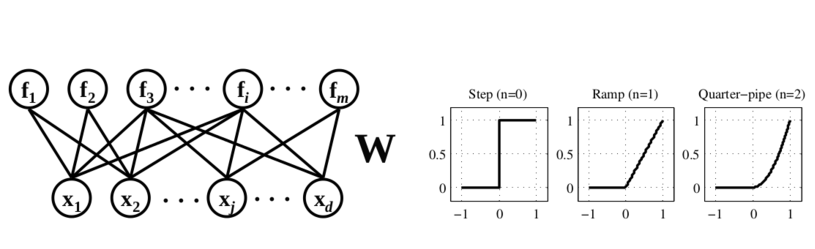
\includegraphics[width=1.0\linewidth, height=7cm]{singnet}
\end{figure}
\end{frame}

\begin{frame}
\frametitle{Multi-layer Arc-cosine Kernel}
Let $f(x)$ and $f(y)$ be the outputs corresponding to inputs $x$ and $y$. Then
\[ f(x)\cdot f(y) = \sum_{i=1}^m \Theta(w_i\cdot x) \Theta(w_i\cdot y)(w_i\cdot x)^n (w_i\cdot y)^n\]
\begin{itemize}
\item $w_i$ = the $i^{th}$ row of weight matrix $W$. 
\item  $m$ = the number of output units.
\end{itemize}
Assume $W_{ij}$ are Gaussian distributed with zero mean and unit variance and the network has an infinite number of output units. Then
\[ lim_{m\rightarrow \infty} \frac{2}{m}f(x)\cdot f(y) = k_n(x,y) \]
\[ k_n(x,y) = 2\int dw \frac{e^{-\frac{\left \| w^2 \right \|}{2}}}{(2\pi )^{d/2}} \Theta (w\cdot x) \Theta (w\cdot y) (w\cdot x)^n (w\cdot y)^n\]
\end{frame}

\begin{frame}
\frametitle{Multi-layer Arc-cosine Kernel}
It has an alternate form
\[ k_n(x,y) = \frac{1}{\pi}\left \| x \right \|^n \left \| y \right \|^n J_n(\theta) \]
where
\[ J_n(\theta) = (-1)^n(sin\theta)^{2n+1} \left ( \frac{1}{sin\theta} \frac{\partial}{\partial \theta} \right )^n \left ( \frac{\pi-\theta}{sin\theta} \right ) \]
n is called the \textbf{degree of the kernel} and
\[ \theta = cos^{-1}\left ( \frac{x\cdot y}{\left \| x \right \| \left \| y \right \|} \right ) \]
\end{frame}

\begin{frame}
\frametitle{Multi-layer Arc-cosine Kernel}
$J_n(\theta)$ for n=0,1,2 is computed as shown below.
\[ J_0(\theta) = \pi-\theta \]
\[ J_1(\theta) = sin\theta + (\pi-\theta)cos\theta \]
\[ J_2(\theta) = 3sin\theta cos\theta + (\pi-\theta)(1+2cos^2\theta) \]
for n=0, it takes the simple form
\[k_0(x,y) =  1- \frac{1}{\pi}cos^{-1}\left ( \frac{x\cdot y}{\left \| x \right \| \left \| y \right \|} \right )  \]
hence the name Arc-cosine kernel is given!
\end{frame}

\begin{frame}
\frametitle{Multi-layer Arc-cosine Kernel}
Multi-layer composition is computed recursively in arc-cosine kernel
\[ k^{(L+1)}_n(x,y) = \frac{1}{\pi} \Bigg[ k^{(L)}(x,x) \textrm{ } k^{(L)}(y,y)\Bigg]^{\frac{n}{2}} J_n(\theta_n^{(L)}) \]
$\theta_n^{(L)}$ =  the angle between images of $x \textrm{ and } y$ in the feature space after L layer composition
\[ \theta_n^{(L)} = \textrm{cos}^{-1}\Bigg( k^{(L)}(x,y) \Bigg[ k^{(L)}(x,x) \textrm{ } k^{(L)}(y,y)\Bigg]^{\frac{-1}{2}} \Bigg) \]
\end{frame}

\begin{frame}
\frametitle{Multi-layer Arc-cosine Kernel}
\begin{block}{Intuition}
if the base kernel $k(x,y) = \phi(x) \cdot \phi(y)$ can mimic the computation of single-layer network, then the iterated mapping in $k^{(L)}(x,y)$ can mimic the computation of multi-layer network.
\end{block}
\end{frame}

\begin{frame}
\frametitle{Multi-layer Kernel Machines}
MKMs are a new family of deep learning algorithm with \textit{kernel methods}.\\
In each layer we perform
\begin{itemize}
\item unsupervised feature extraction with KPCA.
\item a supervised feature selection.
\end{itemize}
\begin{figure}[h]
  \centering
  \captionsetup{justification=centering,margin=0.1cm}
  \includegraphics[scale=0.35]{figures/mkm}
\end{figure}
\end{frame}

\begin{frame}
\frametitle{Multi-layer Kernel Machines}
\renewcommand{\arraystretch}{1.9}
\begin{table}
\centering
\scalebox{0.8}{
\begin{tabular}{|c|c|c|c|c|c|c|c|}
  \hline
  \multirow{2}{*}{\textbf{Dataset}} & \multicolumn{7}{ |c| }{\textbf{Loss in Percentage}} \\
  \cline{2-8}
  & $\textrm{SVM}_{\textrm{RBF}}$ & $\textrm{SVM}_{\textrm{Poly}}$ & NNet & DBN-3 & SAA-3 & DBN-1 & MKMs\\
  \hline  
  \textit{back-rand} & 14.58 & 16.62 & 20.04 & \textbf{6.73} & 11.28 & 9.80 & 10.55\\
  \hline
  \textit{back-image} & 22.61 & 24.01 & 27.41 & 16.31 & 23.00 & \textbf{16.15} & 21.39\\
  \hline
  \textit{rot-back-image} & 55.18 & 56.41 & 62.16 & \textbf{47.39} & 51.93 & 52.21 & 51.61\\
  \hline
  \textit{rect-image} & 24.04 & 24.05 & 33.20 & 23.69 & 24.05 & \textbf{22.50} & 23.01\\
  \hline
\end{tabular}
}
\caption{Experimental Results of MKMs with Arc-cosine Kernels}
\label{tab_results_mkm}
\end{table}
\renewcommand{\arraystretch}{1}
\end{frame}

\begin{frame}
\frametitle{Multi-layer Kernel Machines}
Compared to DBN:\\
\vspace{0.2in}
\begin{itemize}
\setlength\itemsep{1em}
\item MKMs are non-parametric, whereas DBN is parametric. DBN requires to learn millions of parameters to learn and hence computationally expensive.
\item MKMs have no difficult optimization as compared to DBN. 
\end{itemize}
\end{frame}

\begin{frame}
\frametitle{Multi-layer Kernel Machines}
\begin{figure}
  \centering
  \captionsetup{justification=centering,margin=0.1cm}
  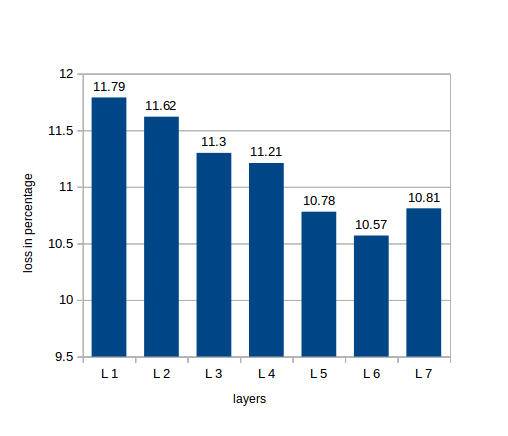
\includegraphics[scale=0.45]{mkm_rand}
  \caption{classifier performance on \textit{mnist-back-rand} dataset.}
  \label{mkm_rand}
\end{figure}
\end{frame}

\begin{frame}
\frametitle{Multi-layer Kernel Machines}
\begin{figure}
  \centering
  \captionsetup{justification=centering,margin=0.1cm}
  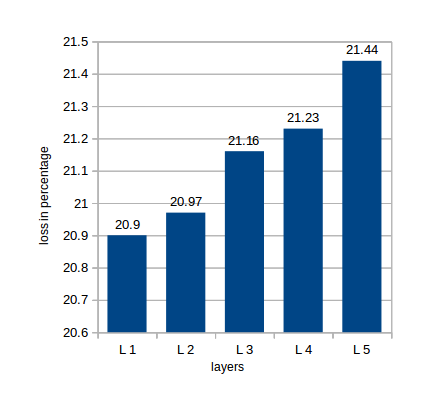
\includegraphics[scale=0.45]{mkm_image}
  \caption{classifier performance on \textit{mnist-back-image} dataset.}
  \label{mkm_image}
\end{figure}
\end{frame}

\begin{frame}
\frametitle{Multi-layer Mixed Kernel Machines}
The architecture of the system is the same as MKMs, but different kernels are used in different layers.\\
\vspace{0.3in}
Empirically, mixing a gaussian/polynomial kernel in between arc-cosine kernels gives the best result.
\end{frame}

\begin{frame}
\frametitle{Multi-layer Mixed Kernel Machines}
\renewcommand{\arraystretch}{1.9}
\begin{table}
\centering
\scalebox{0.8}{
\begin{tabular}{|c|c|c|c|c|c|c|c|}
  \hline
  \multirow{2}{*}{\textbf{Dataset}} & \multicolumn{7}{ |c| }{\textbf{Loss in Percentage}} \\
  \cline{2-8}
  & $\textrm{SVM}_{\textrm{RBF}}$ & $\textrm{SVM}_{\textrm{Poly}}$ & NNet & DBN-3 & SAA-3 & DBN-1 & MKMs(mix)\\
  \hline  
  \textit{back-rand} & 14.58 & 16.62 & 20.04 & \textbf{6.73} & 11.28 & 9.80 & 9.54\\
  \hline
  \textit{back-image} & 22.61 & 24.01 & 27.41 & 16.31 & 23.00 & \textbf{16.15} & 20.94\\
  \hline
  \textit{rot-back-image} & 55.18 & 56.41 & 62.16 & \textbf{47.39} & 51.93 & 52.21 & 54.03\\
  \hline
  \textit{rect-image} & 24.04 & 24.05 & 33.20 & 23.69 & 24.05 & \textbf{22.50} & 25.04\\
  \hline
\end{tabular}
}
\caption{Experimental Results of MKMs with Mixed Kernels}
\label{tab_results_mix}
\end{table}
\renewcommand{\arraystretch}{1}
\end{frame}

\begin{frame}
\frametitle{Multi-layer Multiple Kernel Learning}
Multiple Kernel Learning(MKL) : automate the process of choosing optimum kernel
for the learning task.
\begin{equation*}
\min_{k \in \mathcal{K}} \min_{f \in \mathcal{H}_k} \lambda \norm{f}^2_{\mathcal{H}_k} + \sum_{i=1}^n l(y_i, f(x_i))
\end{equation*}
$l(\cdot) \rightarrow $ the loss function\\
$\mathcal{H}_k \rightarrow $ the RKHS corresponding to the kernel $k \in \mathcal{K}$.
\[ \mathcal{K} = \Bigg\{ k( \cdot \textrm{ , } \cdot ) = \sum_{t=1}^m \mu_t k_t(\cdot \textrm{ , } \cdot) \textrm{ : } \sum_{t=1}^m \mu_t = 1, \mu_t \geq 0 \Bigg\} \]
\end{frame}

\begin{frame}
\frametitle{Unsupervised MKL}
In MKMs we took a combination of kernels in each layer with unsupervised MKL.\\
For finding optimum kernel two quality criteria are used.
\begin{itemize}
\item A  good kernel should enable each training instances to be well reconstructed from the localized bases weighted by the kernel values. ie, for each $x_i$,  $\norm{x_i-\sum_j k_{ij}x_j}^2$, where $k_{ij} = k(x_i, x_j)$, should be minimum.
\item A good kernel should induce kernel values that are coincided with the local geometry of the training data. That is equivalent to minimizing the distortion over all training data $\sum_{i,j}k_{ij} \norm{x_i-x_j}^2 $.
\end{itemize}
\end{frame}

\begin{frame}
\frametitle{Unsupervised MKL}
The cost function
\[ \min_{k \in \mathcal{K}} \frac{1}{2}\sum_{i=1}^n \norm{x_i - \sum_{x_j \in B_i} k_{ij}x_j}^2 + \gamma* \sum_{i=1}^n \sum_{x_j \in B_i} k_{ij} \norm{x_i-x_j}^2 \]
$\gamma$ is a tuning parameter($\gamma$ $>$ 0).
\end{frame}

\begin{frame}
\frametitle{Unsupervised MKL}
The cost function can be converted into a convex QP problem w.r.to kernel weitghts $\mu$.
\begin{equation*}
J(\mu) = \mu^T \Bigg( \sum_{t=1}^m \sum_{i=1}^n k_{t,i}k_{t,i}^T \circ d_i d_i^T \circ P \Bigg)^T \mu + z^T \mu 
\end{equation*}
where $[z]_t = \sum_{i=1}^n (2 \gamma v_i \circ d_i - 2 p_i \circ d_i)^T \mathit{k}_{t,i} $, $P = X^TX$, and $\mathit{k}_{t,i} = \Big[ k^t(x_i, x_1), \ldots, k^t(x_i, x_n) \Big]^T $ is the $i^{th}$ column of the $t^{th}$ kernel matrix. $p$ and $v$ are columns of $P$ and $M$ corresponding to $x_i$ respectively. M is defined as
\[ [M]_{ij} = x_i^Tx_i + x_j^Tx_j - 2x_i^Tx_j \]
\end{frame}

\begin{frame}
\frametitle{Unsupervised MKL}
\begin{figure}
  \centering
  \captionsetup{justification=centering,margin=0.1cm}
  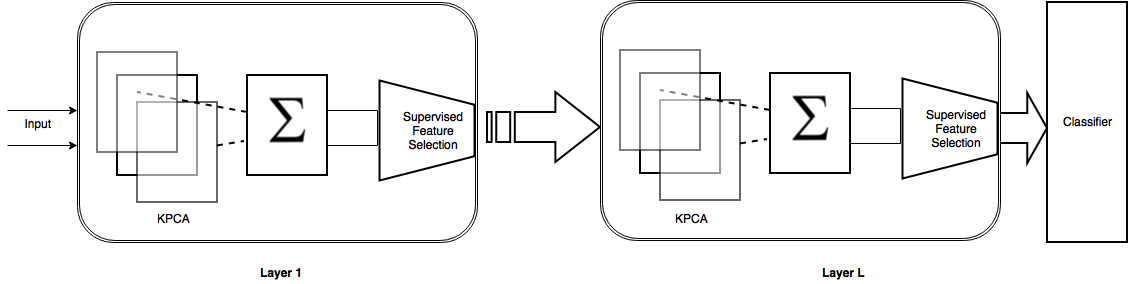
\includegraphics[width=0.9\textwidth,height=4cm]{mlmkm}
  \caption{ML-MKL architecture}
\end{figure}
\end{frame}

\begin{frame}
\frametitle{Unsupervised MKL}
\scalebox{.8}{
\begin{algorithm}[H]
\caption{ML-MKL Algorithm}
\textbf{Input}: data X, true labels y, number of layers L, base kernels for each layer $K_{base}^{(l)} = \{k_1^{(l)}, k_2^{(l)}, k_m^{(l)}\}$, $N_B$, $\gamma$\;
\textbf{Output}: kernel weights $\mu^l$ for each layer, predicted labels\;
1.Initialize $[M]_{ij} = x_i^Tx_i + x_j^Tx_j - 2x_i^Tx_j$, $\bm{D} = d_1, d_2, \ldots, d_n$ as row vectors, where $d_i = \{1 \textrm{ if } x_j \in B_i \textrm{ else } 0 \forall x_j \in X \}$, $\mu = \frac{1}{m}$, $\bm{P} = X^TX$\;
2.\For{each layer l}{
    a. $\bm{W} = \sum_{t=1}^m \sum_{i=1}^n k_{t,i}^{(l)}k_{t,i}^{(l)^{T}} \circ d_i d_i^T \circ P$\\
    b. $\bm{[z]}_t^l = \sum_{i=1}^n (2 \gamma v_i \circ d_i - 2 p_i \circ d_i)^T \mathit{k}_{t,i}^{(l)}$\\
    c. $\bm{\mu}^{*^{l}} = \mu^{l^{T}}W\mu^l + z^{l^{T}}\mu^l$\\
    d. $\bm{K}_{new} = \sum_{t=1}^m \mu_t^l * K_t^{(l)}$\\
    e. extract principal components with $\bm{K}_{new}$\\
    f. select most informative features for layer $l$($X_{new}$)\\
    g. $\bm{P} = X_{new} ^T X_{new}$
}
3.Give the final set of features to any classifier\;
\end{algorithm}
}
\end{frame}

\begin{frame}
\frametitle{Experimental Results}
\renewcommand{\arraystretch}{2.1}
\begin{table}
\centering
\scalebox{.8}{
\begin{tabular}{|c|c|c|c|c|c|c|c|}
  \hline
  \multirow{2}{*}{\textbf{Dataset}} & \multicolumn{7}{ |c| }{\textbf{Loss in Percentage}} \\
  \cline{2-8}
  &$\textrm{SVM}_{\textrm{RBF}}$ & $\textrm{SVM}_{\textrm{Poly}}$ & NNet & DBN-3 & SAA-3 & DBN-1 & \textbf{ML-MKL}\\
  \hline  
  \textit{back-rand} & 14.58 & 16.62 & 20.04 & \textbf{6.73} & 11.28 & 9.80 & 8.43$\pm 0.088$\\
  \hline
  \textit{back-image} & 22.61 & 24.01 & 27.41 & 16.31 & 23.00 & \textbf{16.15} & 20.92$\pm 0.092$\\
  \hline
  \textit{rot-back-image} & 55.18 & 56.41 & 62.16 & \textbf{47.39} & 51.93 & 52.21 & 51.21$\pm 0.811$\\
  \hline
  \textit{rect-image} & 24.04 & 24.05 & 33.20 & 23.69 & 24.05 & \textbf{22.50} & 22.88$\pm 0.124$\\
  \hline
\end{tabular}
}
\caption{Experimental Results of ML-MKL.}
\label{tab_mlmkl}
\end{table}
\renewcommand{\arraystretch}{1}
\end{frame}

\begin{frame}
\frametitle{Experimental Results}
\begin{figure}
  \centering
  \captionsetup{justification=centering,margin=0.1cm}
  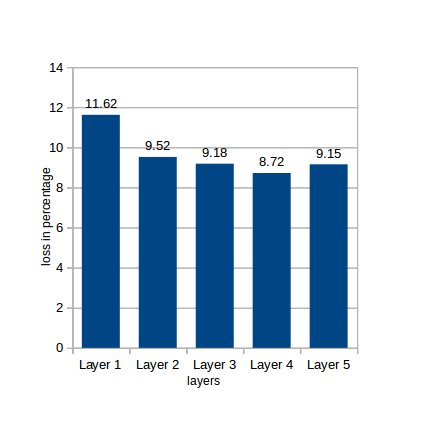
\includegraphics[scale=0.5]{mlmkl_rand}
  \caption{classifier performance on \textit{mnist-back-rand} dataset in each layer.}
  \label{fig_mbr_layers}
\end{figure}
\end{frame}

\begin{frame}
\frametitle{Experimental Results}
\begin{figure}
  \centering
  \captionsetup{justification=centering,margin=0.1cm}
  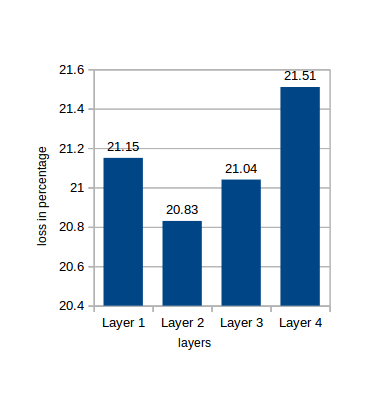
\includegraphics[scale=0.5]{mlmkl_image}
  \caption{classifier performance on \textit{mnist-back-image} dataset in each layer.}
  \label{fig_mbi_layers}
\end{figure}
\end{frame}

\begin{frame}
\frametitle{Experimental Results}
\renewcommand{\arraystretch}{2.1}
\begin{table}
\centering
\scalebox{0.8}{
\begin{tabular}{|c|c|c|c|c|c|c|c|c|}
  \hline
  \multirow{2}{*}{\textbf{Layers}} & \multicolumn{8}{ |c| }{\textbf{Loss in Percentage}} \\
  \cline{2-9}
  & $k_1$ & $k_2$ & $k_3$ & $k_4$ & $k_5$ & $k_6$ & $k_7$ & $K_{conv}$\\
  \hline  
  \textit{Layer 1} & 11.46 & 9.92 & 10.06 & 10.04 & 10.1 & 9.87 & 10.06 & 11.62\\
  \hline
  \textit{Layer 2} & 10.36 & 9.87 & 9.90 & 9.89 & 9.92 & 9.82 & 9.81 & 9.52\\
  \hline
  \textit{Layer 3} & 9.46 & 11.07 & 10.33 & 9.85 & 9.70 & 9.56 & 9.01 & 9.18\\
  \hline
  \textit{Layer 4} & 9.26 & 9.06 & 8.95 & 8.96 & 8.93 & 8.72 & 9.00 & \textbf{8.72}\\
  \hline
  \textit{Layer 5} & 9.18 & 9.07 & 9.02 & 9.20 & 9.22 & 9.36 & 9.47 & 9.15\\
  \hline    
\end{tabular}
}
\caption{Individual kernels performance evaluation for \textit{mnist-back-rand} dataset.}
\label{back_rand_exp}
\end{table}
\renewcommand{\arraystretch}{1}
\end{frame}

\begin{frame}
\frametitle{Experimental Results}
\renewcommand{\arraystretch}{2.1}
\begin{table}
\centering
\scalebox{0.8}{
\begin{tabular}{|c|c|c|c|c|c|c|}
  \hline
  \multirow{2}{*}{\textbf{Layers}} & \multicolumn{6}{ |c| }{\textbf{Loss in Percentage}} \\
  \cline{2-7}
  & $k_1$ & $k_2$ & $k_3$ & $k_4$ & $k_5$ & $K_{conv}$\\
  \hline  
  \textit{Layer 1} & 20.91 & 21.82 & 21.82 & 21.83 & 21.77 & 21.15\\
  \hline
  \textit{Layer 2} & 21.27 & 21.00 & 21.09 & 21.04 & 21.04 & \textbf{20.83}\\
  \hline
  \textit{Layer 3} & 20.95 & 21.18 & 21.02 & 20.99 & 21.05 & 21.03\\
  \hline
  \textit{Layer 4} & 21.06 & 21.36 & 21.42 & 21.64 & 21.66 & 21.51\\
  \hline
\end{tabular}
}
\caption{Individual kernels performance evaluation for \textit{mnist-back-image} dataset.}
\label{back_image_exp}
\end{table}
\renewcommand{\arraystretch}{1}
\end{frame}
%\subsection{Subsection Example} % A subsection can be created just before a set of slides with a common theme to further break down your presentation into chunks

\section{Multi-layer Kernels in Supervised Settings}
\begin{frame}
\frametitle{Kernel Fisher Discriminant Analysis}
\textbf{FDA}: Aims to find a set of features that discriminates the classes very well(works in input space).\\
\textbf{KFDA}: non-linear generalization of FDA(works in RKHS).\\
\vspace{0.3in}
Let $X_1 = \{x_1^1, \ldots, x_{n_1}^1 \}$ and $X_2 = \{x_1^2, \ldots, x_{n_1}^2 \}$ be data samples from two classes (class 1 and class 2). KFDA find the directions $f$ which maximizes the cost function
\begin{equation*}
\mathcal{J}(f) = \frac{f^TS_B^{\phi}f}{f^TS_W^{\phi}f} 
\label{4_jw}
\end{equation*}
\end{frame}


\begin{frame}
\frametitle{Kernel Fisher Discriminant Analysis}
$S_B^{\phi}$ and $S_W^{\phi}$ are the between and within class scatter matrices respectively
\[ S_B^{\phi} = (m_1^{\phi} - m_2^{\phi})(m_1^{\phi} - m_2^{\phi})^T \]
\[ S_W^{\phi} = \sum_{i=1,2}\sum_{x \in X_i} (\phi(x)-m_i^{\phi})(\phi(x)-m_i^{\phi})^T  \]
where $m_i^{\phi} = \frac{1}{n_i} \sum_{j=1}^{n_i} \phi(x_j^i)$.\\
\vspace{0.2in}
\begin{block}{Intuition}
maximizing $\mathcal{J}(f)$ is equivalent to finding a direction $f$ which maximizes the separation of the two classes while minimizing the within class variance.
\end{block}
\end{frame}

\begin{frame}
\frametitle{Kernel Fisher Discriminant Analysis}
we have
\begin{equation*}
f = \sum_{i=1}^n \alpha_i \phi(x_i)
\end{equation*}
applying it in $\mathcal{J}(f)$, we get
\[ f^T S_B^{\phi} f = \alpha^T M \alpha \]
\[ f^T S_W^{\phi} f = \alpha^T N \alpha \] \\
\vspace{0.2in}
where $M = (M_1-M_2)(M_1-M_2)^T$ and $(M_i)_j = \frac{1}{n_i} \sum_{k=1}^{n_i}  k(x_j, x_k^i)$.
\end{frame}

\begin{frame}
\frametitle{Kernel Fisher Discriminant Analysis}
$N = \sum_{i=1,2} K_i(I - \bm{1}_{n_i})K_i^T $, $K_i$ is an $n \times n_i$ matrix with entries $(K_i)_{nm} = k(x_n, x_m^i)$(kernel matrix for class $i$) \\
$I$ is the identity matrix.\\
$\bm{1}_{n_i}$ is the matrix with with all entries $\frac{1}{n_i}$\\
\vspace{0.2in}
Then the cost function can be formulated in terms of $\alpha$
\[ \mathcal{J}(\alpha) = \frac{\alpha^T M \alpha}{\alpha^T N \alpha}  \]
\end{frame}

\begin{frame}
\frametitle{Kernel Fisher Discriminant Analysis}
\renewcommand{\arraystretch}{2.1}
\begin{table}
\centering
\scalebox{0.8}{
\begin{tabular}{|c|c|c|c|c|c|c|c|}
  \hline
  \multirow{2}{*}{\textbf{Dataset}} & \multicolumn{7}{ |c| }{\textbf{Loss in Percentage}} \\
  \cline{2-8}
  &$\textrm{SVM}_{\textrm{RBF}}$ & $\textrm{SVM}_{\textrm{Poly}}$ & NNet & DBN-3 & SAA-3 & DBN-1 & \textbf{KFDA}\\
  \hline  
  \textit{rect-image} & 24.04 & 24.05 & 33.20 & 23.69 & 24.05 & 22.50 & \textbf{21.96}\\
  \hline
  \textit{convex} & 19.13 & 19.82 & 32.25 & 19.92 & \textbf{18.41} & 18.63 & 19.02\\
  \hline
\end{tabular}
}
\caption{Experimental Results of KFDA with multi-layer kernels.}
\end{table}
\renewcommand{\arraystretch}{1}
\end{frame}
%------------------------------------------------

%------------------------------------------------
%------------------------------------------------
\begin{frame}
\frametitle{Multi-layer Kernel on Structured Learning Problems}
Objective : learning a function
\[ h: \mathcal{X} \longrightarrow \mathcal{Y} \]
where $\mathcal{X}$ is the input space and $\mathcal{Y}$ is the output space(structured). To learn $h$, we assume that a training sample of input-output pairs
\[ S = ((x_1, y_1), \ldots, (x_m, y_m)) \in (\mathcal{X} \times \mathcal{Y})^m \]
is available and drawn i.i.d from a distribution P(X,Y).\\
\vspace{0.2in}
We find an $h \in \mathcal{H}$ that minimizes the empirical risk(ERM)
\[ R_s^{\bigtriangleup} = \frac{1}{m} \sum_{i=1}^m \bigtriangleup(y_i, h(x_i)) \]
\end{frame}


\begin{frame}
\frametitle{StructSVM : Problem Formulation}
Here $\bigtriangleup(y, \overline{y})$ denotes the \textbf{loss} associated with predicting $\overline{y}$ when $y$ is the correct output. We assume $\bigtriangleup(y,y) = 0 $ and 
\[ \bigtriangleup(y, \overline{y}) \geq 0 \textrm{ for } y \neq \overline{y} \]
\begin{block}{Method}
StructSVM selects an $h \in \mathcal{H}$ that minimizes a regularized empirical risk\\
on $S$. The general idea here is to learn a discriminant function $\mathnormal{f} : \mathcal{X} \times \mathcal{Y} \longrightarrow \mathbb{R}$ over input/output pairs from which one derives a prediction by maximizing $\mathnormal{f}$ over all $y \in \mathcal{Y}$ for a given input $x$.
\end{block}
\[ h_w(x) =  \underset{y \in \mathcal{Y}}{\arg\max} \mathnormal{f}_w(x,y) \]
We assume $\mathnormal{f}_w(x,y)$ takes a linear form
\[ \mathnormal{f}_w(x,y) = \langle w , \Psi(x,y) \rangle \]
\end{frame}

\begin{frame}
\frametitle{StructSVM : Problem Formulation}
Here $w \in \mathbb{R}^N$ is a parameter vector and $\Psi(x,y)$ is a \textbf{combined feature space} relating input $x$ and output $y$.
\begin{block}{Inuitive picture for $\mathnormal{f}_w(x,y)$}
We can think of $\mathnormal{f}_w(x,y)$ as a compatibility function that measures how well the output $y$ matches the given input $x$.
\end{block}
\vspace{0.2in}
$\Psi(x,y)$ has to be defined specific to problems(Natural Language Parsing(NLP), Protein Sequence Alignment, Image Segmentation etc).\\
\end{frame}

\begin{frame}
\frametitle{StructSVM : Problem Formulation}
1. \textbf{Margin Rescaling}(MR)\\
In MR the position of the hinge is adapted keeping the slope fixed. 
\[ \bigtriangleup_{MR}(y, h_w(x)) =  \underset{\overline{y} \in \mathcal{Y}}{\max}\{ \bigtriangleup(y, \overline{y}) - \langle w , \Psi(x,y) \rangle + \langle w , \Psi(x,\overline{y}) \rangle \} \]
\[ \geq \bigtriangleup(y, h_w(x)) \] \\
\vspace{0.2in}
1. \textbf{Slack Rescaling}(SR)\\
In SR the slope is adjusted while keeping the position of the hinge fixed.
\[ \bigtriangleup_{SR}(y, h_w(x)) =  \underset{\overline{y} \in \mathcal{Y}}{\max}\{ \bigtriangleup(y, \overline{y})(1 - \langle w , \Psi(x,y) \rangle + \langle w , \Psi(x,\overline{y}) \rangle) \} \]
\[ \geq \bigtriangleup(y, h_w(x)) \]
\end{frame}


\begin{frame}
\frametitle{StructSVM : Problem Formulation}
\begin{block}{n-Slack StructSVM with Margin Rescaling}
\[\underset{w, \xi \geq 0}{\min} \quad \frac{1}{2} \norm{w}^2 + \frac{C}{m} \sum_{i=1}^m \xi_i \]
\[ \textrm{s.t } \forall \overline{y_1} \in \mathcal{Y} \textrm{  :  } w^T[\Psi(x_1, y_1) - \Psi(x_1, \overline{y_1})] \geq \bigtriangleup(y_1, \overline{y_1}) - \xi_1 \]
\[ \vdots \]
\[ \textrm{s.t } \forall \overline{y_m} \in \mathcal{Y} \textrm{  :  } w^T[\Psi(x_m, y_m) - \Psi(x_m, \overline{y_m})] \geq \bigtriangleup(y_m, \overline{y_m}) - \xi_m \]
\end{block}

\end{frame}

\begin{frame}
\frametitle{StructSVM : Problem Formulation}
\begin{block}{n-Slack StructSVM with Slack Rescaling}
\[\underset{w, \xi \geq 0}{\min} \quad \frac{1}{2} \norm{w}^2 + \frac{C}{m} \sum_{i=1}^m \xi_i \]
\[ \textrm{s.t } \forall \overline{y_1} \in \mathcal{Y} \textrm{  :  } w^T[\Psi(x_1, y_1) - \Psi(x_1, \overline{y_1})] \geq 1 - \frac{\xi_1}{\bigtriangleup(y_1, \overline{y_1})} \]
\[ \vdots \]
\[ \textrm{s.t } \forall \overline{y_m} \in \mathcal{Y} \textrm{  :  } w^T[\Psi(x_m, y_m) - \Psi(x_m, \overline{y_m})] \geq 1 - \frac{\xi_m}{\bigtriangleup(y_m, \overline{y_m})} \]
\end{block}
The constraints states that for each training example, $(x_i, y_i)$ the score $w^T[\Psi(x_i, y_i)$ must be greater than the score $w^T[\Psi(x_i, \overline{y})$ of all outputs $\overline{y} \in \mathcal{Y}$ by a required margin. This margin is 1 in SR and $\bigtriangleup(y, \overline{y})$ in MR.
\end{frame}

\begin{frame}
\frametitle{StructSVM : Experimental Results}
\renewcommand{\arraystretch}{1.2}
\begin{table}
\centering
\scalebox{0.8}{
\begin{tabular}{|c|c|c|}
	\hline
	\textbf{Dataset} & \textbf{Arc-Cosine Kernel} & \textbf{Other Kernel(best)}\\
	\hline
	Scene Segentation & 30.35 & 30.60 \\
	(multilabel - 6 class) & & \\
	\hline
	Vehicle Dataset & 26.48 & 24.90 \\
	(multiclass - 4 class) & & \\
	\hline
	Iris Dataset & 1.67 & 3.33 \\
	(multiclass - 3 class) & & \\
	\hline
	Breast Cancer Wiscosin & 0.98 & 0.98 \\
	(binary) & & \\
	\hline
	Synthetic Data & 33.85 & 32.55 \\
	(multiclass - 7 class) & & \\
	\hline
\end{tabular}
}
\end{table}
\renewcommand{\arraystretch}{1}
\end{frame}


\section{Conclusion \& Future Plans}

\begin{frame}
\frametitle{Conclusion}
\begin{itemize}
\setlength\itemsep{0.4em}
\item Performance of MKMs are comparable with popular deep learning algorithms like DBN, SAA etc.
\item Using (unsupervised) MKL in MKMs improves the classifier performance.
\item KFDA performs well when using, either a highly non-linear arc-cosine kernel(degree $>$ 1) or a
multi-layer arc-cosine kernel with very large number of layers (above 10).
\item Multi-layer kernels performs competetive with single layer kernel machines on structured output spaces.
\end{itemize}
\end{frame}

\begin{frame}
\frametitle{Future Plans}
\begin{itemize}
\setlength\itemsep{1em}
\item A thoretical study on the optimal structure of ML-MKL model(number of layers required, number of kernels in each layer).
\item Fine-tuning mechanisms for ML-MKL model.
\item Multi-layer kernel can be tested on complex structured output prediction problems like parse tree prediction, protein segment alignment prediction etc.
\end{itemize}
\end{frame}

\begin{frame}
\frametitle{Important References}
\footnotesize{
\begin{thebibliography}{99} % Beamer does not support BibTeX so references must be inserted manually as below
\bibitem[Saul]{p1} Y. Cho, L.K. Saul, Kernel Methods  for Deep Learning
\newblock \emph{Advances in Neural Information Processing Systems(NIPS) 22}, 342 -- 350, 2009.

\bibitem[Zhuang, 2011]{zhuang} J. Zhuang, Jialei Wang, Steven C.H Hoi, Xiangyang Lan, Unsupervised Multiple Kernel Learning. \newblock \emph{Journal of Machine Learning Research(JMLR)} Volume 20, 129--144, 2011.

\bibitem[Sebastian]{kfda} Sebastian Mika, Gunnar R\"{a}tsch, Jason Weston, Bernhard Sch\"{o}lkopf, and Klaus-Robert M\"{u}ller, Fisher Discriminant Analysis With Kernels. \newblock \emph{Journel of Neural Networks for Signal Processing}, pp 41--48, 1999.

\bibitem[Bengio, 2007]{bengioAI} Yoshua Bengio and Yann LeCun, Scaling learning algorithms towards AI.  in Bottou, L. and Chapelle, O. and DeCoste, D. and Weston, J. (Eds) \newblock \emph{Large-Scale Kernel Machines}, MIT Press,  2007.

\bibitem[Bengio, 2013]{bengioRL} Yoshua Bengio, Aaron Courville and Pascal Vincent, Representation Learning: A Review and New Perspectives. \newblock \emph{IEEE Transactions on Pattern Analysis and Machine Intelligence(TPAMI)} Volume 35, 1798--1828, August 2013.

\bibitem[Joachims, 2009]{p1} T. Joachims, T. Finely, C. John Nu, Cutting-Plane Training on Structural SVMs
\newblock \emph{Journal of Machine Learning 77(1)}, 27 -- 59, 2009.

\end{thebibliography}
}
\end{frame}

\iffalse
%commented region

\begin{frame}
\frametitle{Multiple Columns}
\begin{columns}[c] % The "c" option specifies centered vertical alignment while the "t" option is used for top vertical alignment

\column{.45\textwidth} % Left column and width
\textbf{Heading}
\begin{enumerate}
\item Statement
\item Explanation
\item Example
\end{enumerate}

\column{.5\textwidth} % Right column and width
Lorem ipsum dolor sit amet, consectetur adipiscing elit. Integer lectus nisl, ultricies in feugiat rutrum, porttitor sit amet augue. Aliquam ut tortor mauris. Sed volutpat ante purus, quis accumsan dolor.

\end{columns}
\end{frame}

%------------------------------------------------
\section{Second Section}
%------------------------------------------------

\begin{frame}
\frametitle{Table}
\begin{table}
\begin{tabular}{l l l}
\toprule
\textbf{Treatments} & \textbf{Response 1} & \textbf{Response 2}\\
\midrule
Treatment 1 & 0.0003262 & 0.562 \\
Treatment 2 & 0.0015681 & 0.910 \\
Treatment 3 & 0.0009271 & 0.296 \\
\bottomrule
\end{tabular}
\caption{Table caption}
\end{table}
\end{frame}

%------------------------------------------------

\begin{frame}
\frametitle{Theorem}
\begin{theorem}[Mass--energy equivalence]
$E = mc^2$
\end{theorem}
\end{frame}

%------------------------------------------------

\begin{frame}[fragile] % Need to use the fragile option when verbatim is used in the slide
\frametitle{Verbatim}
\begin{example}[Theorem Slide Code]
\begin{verbatim}
\begin{frame}
\frametitle{Theorem}
\begin{theorem}[Mass--energy equivalence]
$E = mc^2$
\end{theorem}
\end{frame}\end{verbatim}
\end{example}
\end{frame}

%------------------------------------------------


%------------------------------------------------

\begin{frame}[fragile] % Need to use the fragile option when verbatim is used in the slide
\frametitle{Citation}
An example of the \verb|\cite| command to cite within the presentation:\\~

This statement requires citation \cite{p1}.
\end{frame}

%------------------------------------------------

\fi

%------------------------------------------------

\begin{frame}
\frametitle{List of papers based on thesis}
1. Akhil P M, Asharaf S, Sumitra S, {\em Unsupervisd MKL in Multi-layer Kernel Machines}(paper under preparation).
\end{frame}


\begin{frame}
%\Huge{\centerline{The End}}
\begin{figure}

\includegraphics[width=0.7\linewidth, height=7.5cm]{figures/thankyou}
\end{figure}
\end{frame}

%----------------------------------------------------------------------------------------

\end{document} 